%!Mode:: "TeX:UTF-8"
%\begin{frame}
%    \frametitle{OUTLINE}
%    \begin{itemize}    
%        \item
%    \end{itemize}
%\end{frame}

\begin{frame}
    \begin{center}
        \LARGE \tt{TRAC}
    \end{center}
\end{frame}

\begin{frame}
    \frametitle{为何用trac?}
    \begin{itemize}    
        \item 目前的地址:
        \item \url{http://dyb2app1.ihep.ac.cn/trac}
        \item 汇总各种信息
            \begin{itemize}
                \item 包括一些Wiki信息
                \item BUG的汇报
                \item 软件的计划
            \end{itemize}
        \item 便于查找相关的内容
        \item 在{\tt ticket}中,大家可以发贴进行交流
    \end{itemize}
    \begin{block}{术语及其作用}
        \begin{description}
            \item[Wiki] 各种知识和信息的表达,例如项目的整体组织情况
            \item[Ticket] 各种问题及目标的报告,可认为是一个事件
            \item[Milestone] 由Ticket组成,查看项目中子单元的进度
        \end{description}
    \end{block}
\end{frame}

\begin{frame}
    \frametitle{Wiki功能}
    \begin{itemize}    
        \item 这里的功能大家自己摸索
        \item 一些有趣的功能
            \begin{itemize}
                \item 插入代码
                \item 可支持
                    \begin{itemize}
                        \item c
                        \item cpp
                        \item python
                        \item 甚至是diff
                    \end{itemize}
                \item Workflow
            \end{itemize}
    \end{itemize}
\end{frame}

\newsavebox{\TracWikiCodeCpp}
\begin{lrbox}{\TracWikiCodeCpp}
\begin{lstlisting}[language=c++]
{{{#!cpp

class A{
};

}}}
\end{lstlisting}
\end{lrbox}

\lstdefinelanguage{diff}{
  morecomment=[f][\color{blue}]{@@},     
  morecomment=[f][\color{red}]-,         
  morecomment=[f][\color{dkgreen}]+,       
  morecomment=[f][\color{red}]{---}, 
  morecomment=[f][\color{dkgreen}]{+++},
}

\newsavebox{\TracWikiCodeDiff}
\begin{lrbox}{\TracWikiCodeDiff}
\begin{lstlisting}[language=diff]
{{{
#!diff
--- Version 55
+++ Version 56
@@ -115,8 +115,9 @@
     name='TracHelloWorld', version='1.0',
     packages=find_packages(exclude=['*.tests*']),
-    entry_points = """
-        [trac.plugins]
-        helloworld = myplugs.helloworld
-    """,
+    entry_points = {
+        'trac.plugins': [
+            'helloworld = myplugs.helloworld',
+        ],
+    },
 )
}}}
\end{lstlisting}
\end{lrbox}

\begin{frame}
    \frametitle{插入代码}
    \begin{block}{\tt{C++}代码}
        \par\usebox{\TracWikiCodeCpp}
    \end{block}
\end{frame}

\begin{frame}
    \frametitle{插入代码}
    \begin{block}{\tt{diff}代码}
        \par\usebox{\TracWikiCodeDiff}
    \end{block}
\end{frame}

\newsavebox{\TracWikiWorkflow}
\begin{lrbox}{\TracWikiWorkflow}
%\begin{adjustbox}{width=\textwidth,height=10cm,keepaspectratio}
\begin{lstlisting}
{{{#!Workflow

read_public_admin = dyb2app1 -> gitadmin
read_public_user = dyb2app1 -> user

read_users_admin = users -> gitadmin
read_users_user = users -> user

write_public_repo = gitadmin -> dyb2app1
write_users_repo = user -> users

}}}
\end{lstlisting}
%\end{adjustbox}
\end{lrbox}

\begin{frame}
    \frametitle{Wiki中Workflow的代码}
    \par\usebox{\TracWikiWorkflow}
\end{frame}

\begin{frame}
    \frametitle{Wiki中Workflow的效果}
    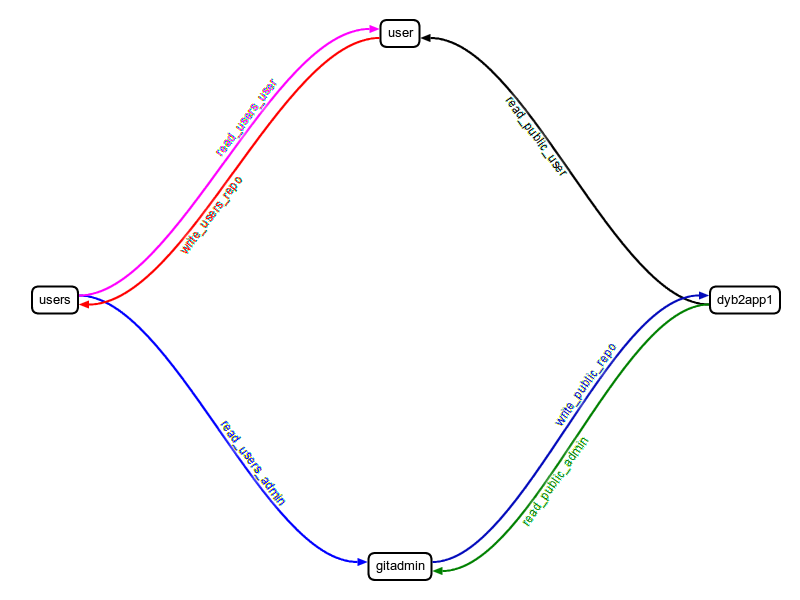
\includegraphics[width=10cm,keepaspectratio]{data/TracWorkflow.png}
\end{frame}


\begin{frame}
    \frametitle{Ticket的用处}
    \begin{itemize}    
        \item 向大家报告程序中的Bug
        \item 搜索有没有类似的Bug
        \item 设定下一步目标
        \item 例如,要进行一个新的探测器原型的开发
            \begin{itemize}
                \item 创建一个ticket,说明目标
                \item 得到的ticket的id
                \item 在个人仓库中建立一个相应ticket的分支
            \end{itemize}
    \end{itemize}
    \begin{block}{关于Ticket ID的妙用}
    \begin{itemize}    
        \item 例如,这个ticket的id为10。
        \item 在wiki中,可以用\tt{\#10}指向这个ticket。
        \item 在\tt{commit}的内容中,也可以
              使用\tt{\#10}。
        \item \tt{\scriptsize{git commit -am "Finish Ticket \#10."}}
        \item 完成后,就将此ticket关闭。
        \item Trac中,自动为\tt\textcolor{red}{{\sout{\#10}}} 创建了链接。
    \end{itemize}
    \end{block}
\end{frame}


\begin{frame}
    \frametitle{创建Ticket}
    \begin{itemize}    
        \item 创建Ticket时,不管是汇报bug,或者是一个新的目标,
              请尽量贴出有用信息,把问题描述清楚。
        \item 另外,好的习惯是,把这个Ticket中的信息补充完整。
        \item 例如,对于component来说,如果在开发DetSimX,
              那么就选择\tt{dyb2sim DetSimX}。
        \item 如果选项中的条目不完善,请告知管理员
        \item 具体的流程,还需要进一步讨论
    \end{itemize}
    \begin{block}{一些选项}
        \begin{description}
            \item[Type] 指定Ticket的类型,例如,{\tt Pull Request}
            \item[Component] 指定此Ticket对应哪块组件,例如{\tt DetSimX}
            \item[Milestone] 指定这个Ticket属于哪个Milestone,
                             例如{\tt "Dyb2 Detector MC"}
            \item[Version] 指定此Ticket针对的版本
        \end{description}
    \end{block}
\end{frame}

\begin{frame}
    \frametitle{Milestone(在Roadmap中)}
    \begin{itemize}    
        \item Trac中的Milestone,不是以一个时间段作为标记。
        \item 而是以完成的Ticket数做为标记。
        \item 因此,ticket中信息填全有助于我们了解项目的进展。
        \item 一个项目只要有进展,最会有新的Ticket出现,
              而又有旧的被关闭。
    \end{itemize}
\end{frame}

\begin{frame}
    \frametitle{Trac小结}
    \begin{itemize}    
        \item 遇到问题时,先搜索有没有类似的问题
        \item 如果能找到,看看是否已经修改了这个bug
        \item 如果没有,请创建新的Ticket,尽快告知大家
        \item 以Ticket的形式,记录新的工作
        \item 与大家分享你的工作进展
    \end{itemize}
\end{frame}
